\documentclass[hoptionsi, twocolumn]{revtex4-2}
\usepackage[english,russian]{babel}
\usepackage[utf8]{inputenc}
\usepackage{natbib}
\usepackage{setspace}
\usepackage{graphicx}
\usepackage{dcolumn}
\usepackage{bm}
\usepackage{geometry}
\usepackage{graphicx}
\usepackage[unicode, pdftex,hidelinks]{hyperref}
\usepackage{amsmath}
\usepackage{float}
\usepackage{amssymb}


\begin{document}

\title{Изучение движения вертикально падающих тел}
\author{Турчанин Е., Солдатова В., Горбушкин Г. и Мнацаканов Ф.}
\affiliation{
 Физический Факультет, Университет ИТМО, \\
 Санкт-Петербург, 199034, Российская Федерация 
}
\author{Гулинян В.}
\affiliation{
 Научный руководитель. Физический Факультет, Университет ИТМО,\\
 Санкт-Петербург, 199034, Российская Федерация
}
\begin{abstract}
 Когда-то появится
\end{abstract}
\maketitle
\onehalfspacing
\twocolumngrid
\section{Введение}
В качестве иллюстрации неинерциальности системы отсчета Земли часто используется хорошо известная задача о горизонтальном отклонении объекта, сброшенного с некоторой высоты. При решении уравнений движения в системе отсчета, связанной с Землей, в уравнения движения вводятся приближения. В результате получается формула для вычисления отклонения вертикально падающего объекта в восточном направлении. Недостатком данного метода является недостаточное физическое объяснение происхождения этих отклонений. Альтернативным решением упомянутой задачи является вывод уравнения траектории движения объекта относительно инерциальной системы отсчета. J. M. Potgieter в  \cite{1} рассматривает участок эллиптической орбиты частицы в инерциальной системе отсчета связанной с Землей, чтобы получить ее отклонение на восток при свободном падении частицы из состоянии покоя. Это отклонение считается от радиального направления. В комментариях к горизонтальному отклонению падающего объекта Elie Belozersky и Jean Sivardiere \cite{3}, поправляя Potigier, находят отклонение вертикально падающего объекта на юг (или север – в зависимости от полушария) от линии отвеса. Также решать проблему вертикально падающего тела можно применяя второй закон Кеплера, как это делает John F. Wild \cite{9} или через закон сохранения момента импульса\cite{6}.

Несмотря на то, что теоретическое отклонение вертикально падающего тела невелико, нахождение этого отклонения представляет практический интерес: на спортивных мероприятиях в некоторых ситуациях необходимо учитывать это отклонение (например –- cпортивная стрельба на большие расстояния), при полете ракет траектория полета имеет отклонение от первоначального направления. Одной из задач проекта является нахождение начальных параметров, при которых смещением можно пренебречь. Кроме того, было изучено падение тел как с нулевой, так и ненулевой начальными скоростями; рассмотрено влияние значения ускорения свободного падения на отклонение тела от вертикали. Результаты для наглядности были получены путем моделирования в Python. 
\section{Теоретическая часть}
В этом разделе мы рассмотрим теоретическое описание движения падающего твердого тела, которое позволит найти зависимость отклонения объекта от различных параметров системы, таких как: начальные скорость и положение тела, масса и радиус планеты. Мы будем использовать дифференциальные уравнения, которые получили Martin S. Tiersten и Harry Soodak \cite{4}:
\begin{equation*}
    \begin{cases}
    \ddot{x} = g_{x, x}x +g_{x,z}z+2\omega_{z}\dot{y}, \\
    \ddot{y} = g_{y, y}y -2\omega_{z}\dot{x} +2\omega_{x}\dot{z}, \\
     \ddot{z} = - g_0+ g_{z, x}x + g_{z, z}z-2\omega_{x}\dot{y}, 
    \end{cases}
\end{equation*}
где
\begin{equation*}
    \begin{aligned}
        &g_{x,x}=-\left(\dfrac{g_{E0}}{R_0}-\omega_z^2\right)=-\left(\dfrac{GM}{R^3_0}-\omega\cos{\theta}\right) =\\
        &= -\dfrac{GM}{R^3_0} +\omega\cos{\left(\psi_0-\dfrac{\omega^2R_0^3}{GM}\sin{\psi_0}\cos{\psi_0}\right)}, \\
        &g_{y,y}=-\left(\dfrac{g_{E0}}{R_0}-\omega_y^2\right)=-\dfrac{GM}{R_0^3}+\omega^2,\\
        &g_{z,z}=2\dfrac{g_{E0}}{R_0}+\omega_x^2=2\dfrac{GM}{R_0^3}+\\
        &+\omega^2\sin^2{\left(\psi_0-\dfrac{\omega^2R_0^3}{GM}\sin{\psi_0}\cos{\psi_0}\right)},\\
          &g_{x,z}=g_{z,x}=3\alpha\dfrac{g_{E0}}{R_0} - \omega_x\omega_z=\\
&=3\alpha\dfrac{GM}{R_0^3}+\dfrac{\omega^2}{2}\sin{\left(2\psi_0-\dfrac{\omega^2R_0^3}{GM}\sin{2\psi_0}\right)},
    \end{aligned}
\end{equation*}
 \begin{equation*}
    \begin{aligned}
&g_{x,y}=g_{y,x}=g_{y,z}=g_{z,y}=0.
    \end{aligned}
\end{equation*}

 C помощью этих уравнений было получено выражение для конечного отклонения тела, брошенного с высоты, при различных начальных условиях.\\
\begin{figure}[h]
\centering
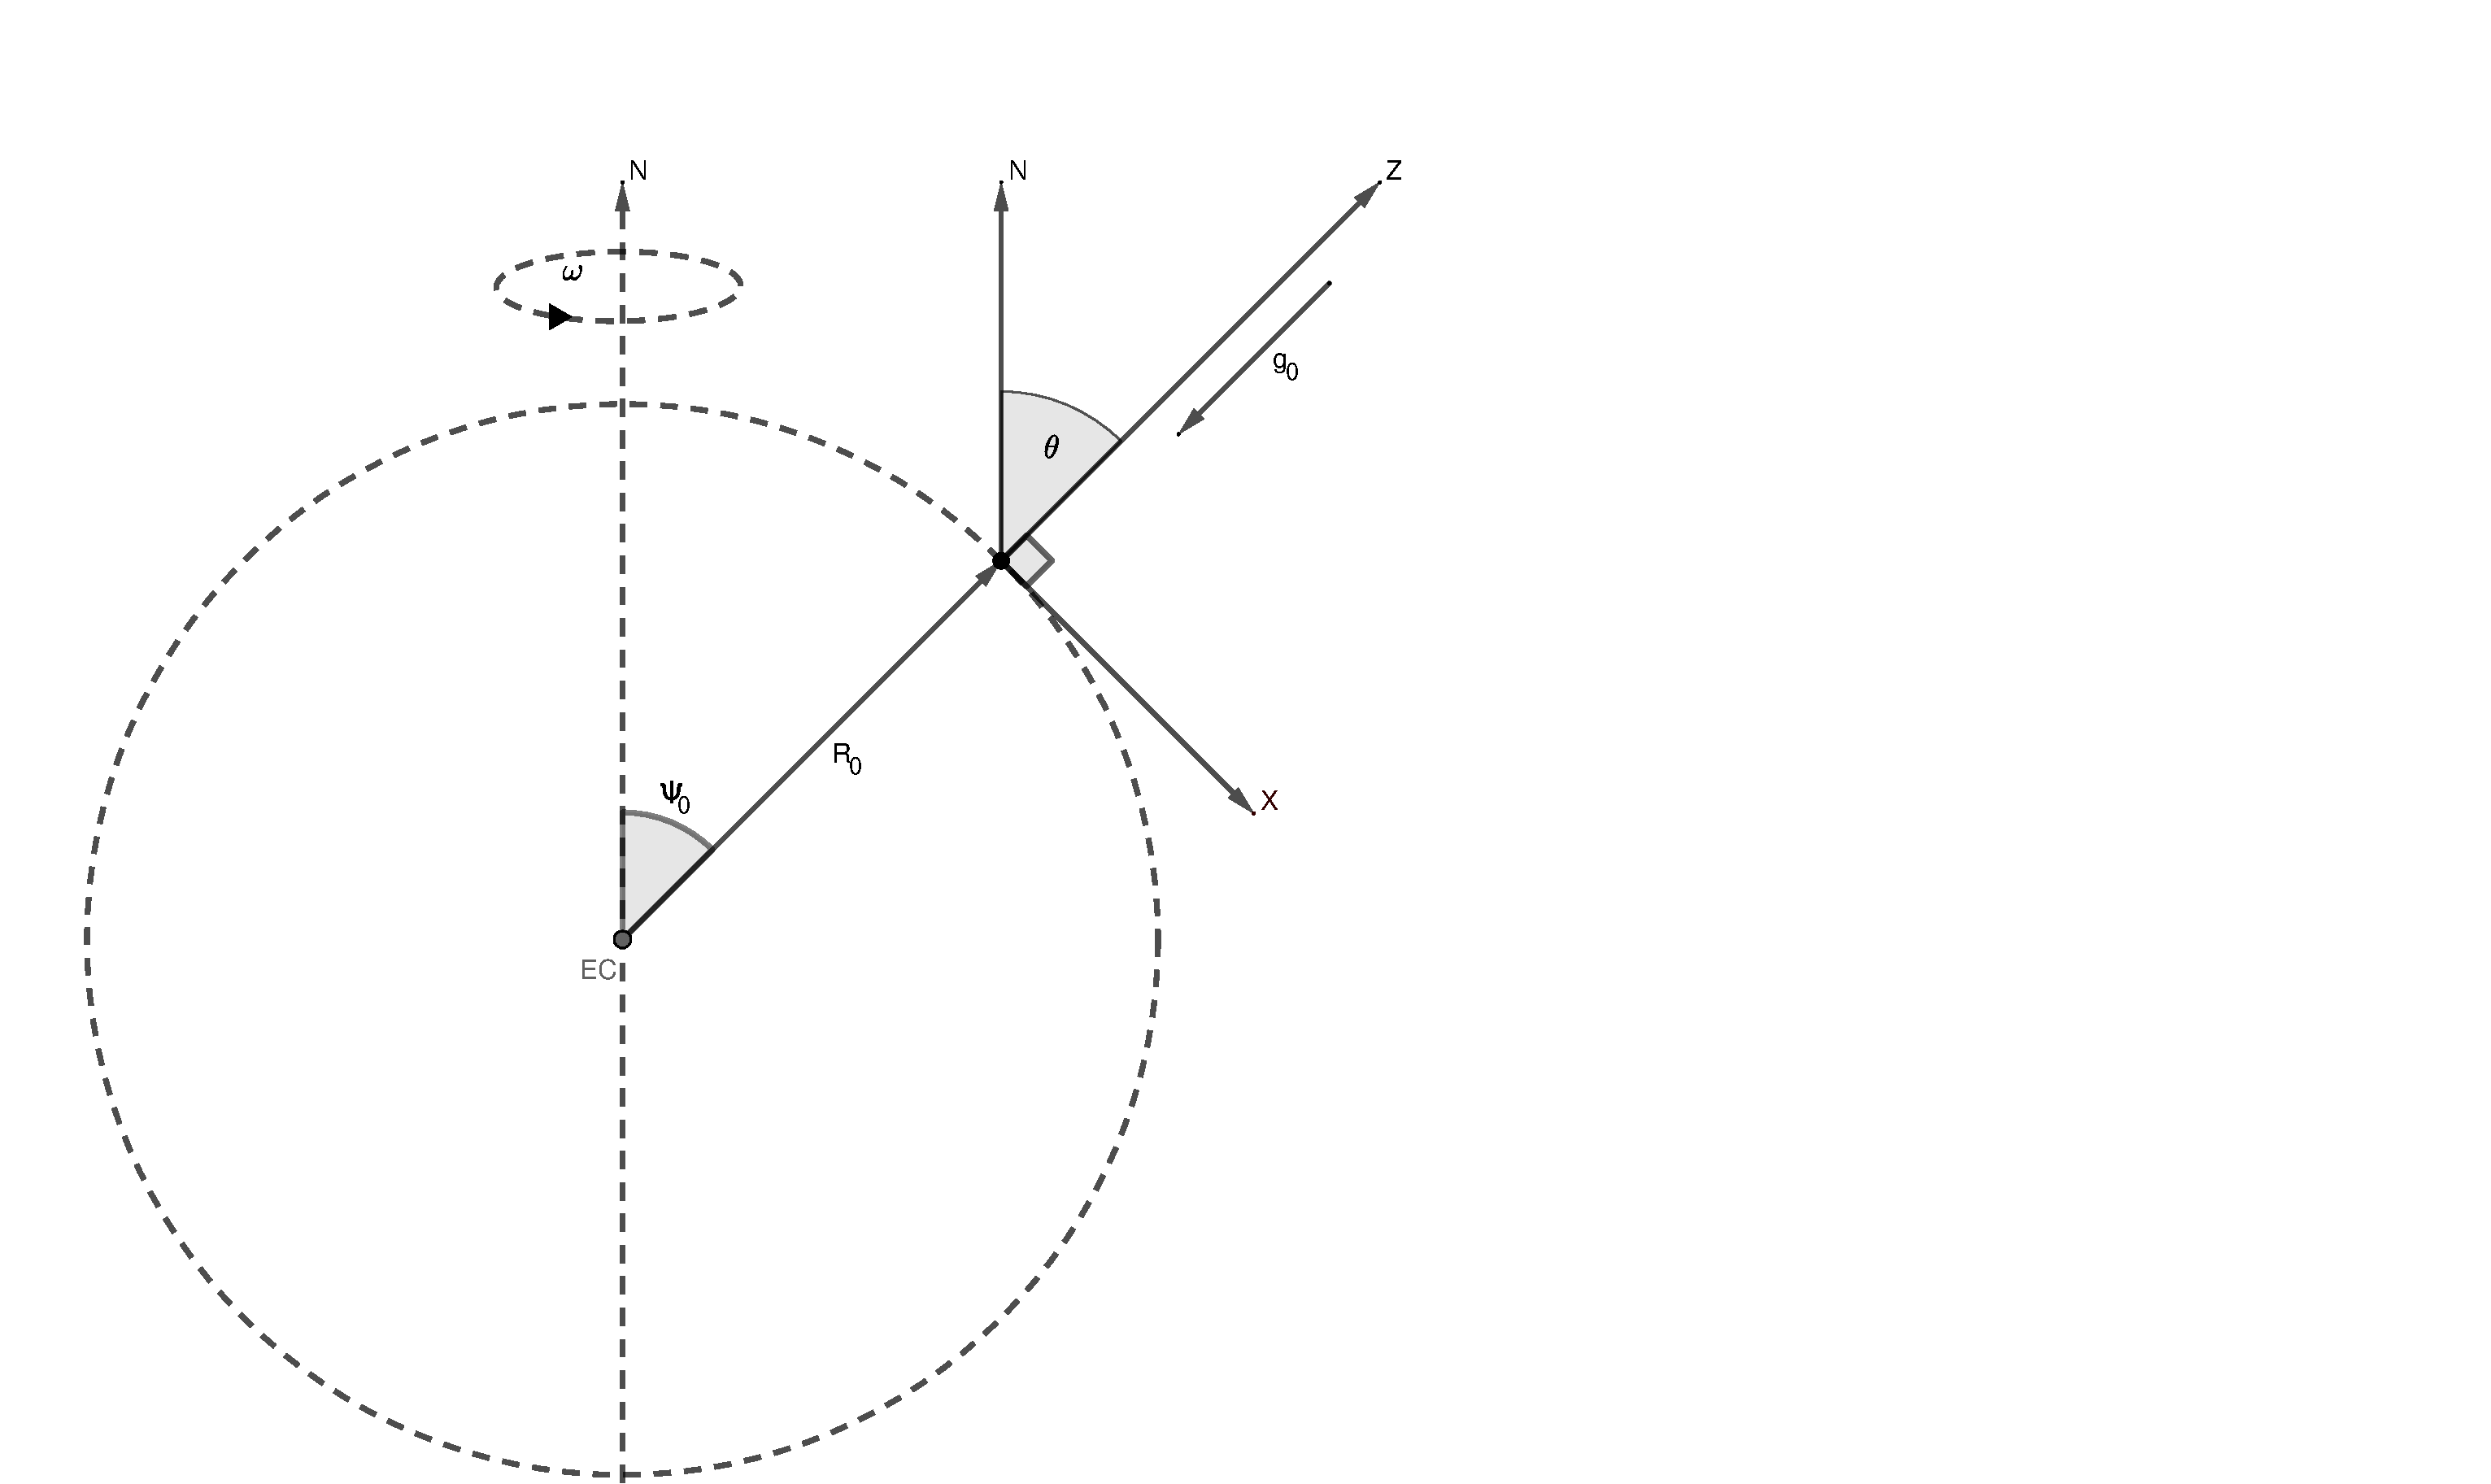
\includegraphics[width=0.4\textwidth]{pick-1.pdf}
\caption{$N$ --- ось вращения планеты, EC --- центр земли, ось $x$ направлена к экватору и  лежит в плоскости, образованной вертикальной осью $z$ и меридианом, который проходит через точку пересечения оси $z$ и поверхностью планеты. Ось $y$ направлена на восток. $\theta$ --- угол между осью вращения $N$ и осью $z$. Местом броска задаются $M$, $R_0$, $\omega$ --- масса, радиус и  угловая скорость вращения планеты соответственно; $\psi_0$ --- угол между северным полюсом и местом броска. $g_0$ --- локальное начальное значение ускорения свободного падения в точке отсчета.}
\label{fig:pick-1}
\end{figure}
В исходной статье рассматривалось падение тела с нулевой начальной скоростью. Цель этой работы получить решения системы с ненулевыми начальными проекциями скорости по осям $x, y, z$. Введем следующие начальные условия:
\begin{equation*}
    \begin{aligned}
        &x =y=0, \qquad z=h,\\
        &\dot x=v_x, \quad \dot y=v_y, \quad \dot z =v_z.
    \end{aligned}
\end{equation*}



В каждой задаче необходимо определиться с желаемой точностью результата. Велечинами какого порядка малости можно пренебрегать для получения более простого решения, чтобы при этом не терять точность результата. В нашей задаче при падении тела с высоты до 100 м, для получения восточного отклонения с высокой точностью необходимо учитывать силу Кориолисса (соответственно, нельзя пренебрегать $\omega$); для учета мередиального отклонения необходимо также учитывать и $g_{x,z}$ (соотвественно, берем в рассчет также и $\omega^2$). Кроме того, т к используется модель идеальной сферической Земли, полученные значения также могут отличаться от реальных.
Количественная обоснованность любого
приближения должна быть установлена посредством покомпонентного анализа, с обязательной проверкой порядков величин и/или
оценкой вклада как сохраненных, так и пренебрегаемых членов в уравнениях, описывающих динамику системы. Далее будет произведена оценка влияния компонент на вертикально падающее тело.

Так как $g_{x, x},\ g_{y, y},\ g_{z, z}\approx 10^{-6}\;1/c^2$, $\omega_z=\omega\cos{\theta}< 10^{-4}\;1/c$. Получаем систему:
\begin{equation*}
    \begin{cases}
    \ddot{x} = g_{x,z}z+2\omega_{z}\dot{y},  \\
    \ddot{y} =2\omega_{x}\dot{z}=2\omega_{x}\left(v_z-g_0t\right),\\
     \ddot{z} = - g_0,
    \end{cases}
\end{equation*}
Интегрируя выражения для $\ddot z$ и $\ddot y$, находим $\dot z$, $z$, $\dot y$ и $y$.
\begin{equation*}
    \begin{aligned}
    & \dot z = v_z-g_0t,\\
    &z = h+v_zt-\dfrac{g_0t^2}{2},\\
    &\dot y = 2\omega_x v_z t-\omega_x g_0t^2+v_y,\\
    &y= 2\omega_x v_z t^2-\dfrac{\omega_x g_0t^3}{3} +v_yt,
    \end{aligned}
\end{equation*}
С этими данными получаем следующие уравнения для $\ddot x$, $\dot x$ и $x$:
\begin{multline*}
    \ddot{x} = g_{x,z}\left(h+v_zt-\dfrac{g_0t^2}{2}\right)+\\
    +2\omega_{z}\left(2\omega_x v_z t-\omega_x g_0t^2 + v_y\right),
\end{multline*}
\begin{multline*}
    \dot{x} = v_x+g_{x,z}\left(ht+\dfrac{v_zt^2}{2}-\dfrac{g_0t^3}{6}\right)+\\
    +2\omega_{z}\left(\omega_x v_z t^2-\dfrac{\omega_x g_0t^3}{3} + v_yt\right),
\end{multline*}
\begin{multline*}
    x=g_{x,z}\left(\dfrac{ht^2}{2}+\dfrac{v_zt^3}{6}-\dfrac{g_0t^4}{24}\right)+\\
    +2\omega_{z}\left(\dfrac{\omega_x v_z t^3}{3}-\dfrac{\omega_x g_0t^4}{12} + \dfrac{v_yt^2}{2}\right)+v_xt.
\end{multline*}
Понятно, что при $z=0$ тело упадет на поверхность планеты. Тогда время его падения:
\[
t=\dfrac{v_z}{g_0}+\dfrac{\sqrt{v_z^2+2g_0h}}{g_0},
\]
подставляем это в выражение для $x$ и $y$, мы получим выражения для нахождения смещения по координатам $x$ и $y$.

Для моделирования использовался язык программирования python, с использованием пакетов numpy, matplotlib, scipy. Для решения дифференциальных уравнений использовался метод DOP853 \cite{dop853}, основная аппроксимация имеет порядок 8, этого достаточно, так как мы смотрим на смещения порядка $10^{-3}$ м. Также метод включает механизм оценки, что дает нам малую ошибку, порядка $O(h^8)$. При помощи метода Рунге-Кутты, на каждом шаге решается дифференциальное уравнение на основе текущего значения $y(t)$, временного шага $h$, и функции $f(t,\;y)$, описывающей уравнение, значение $y(t+h)$ вычисляется с использованием порядка 8, оценивается ошибка с использованием формул порядка 5 и 3, чтобы адаптировать шаг $h$, если ошибка выше заданного порога, шаг уменьшается, если ошибка мала, шаг увеличивается для ускорения вычислений.\onecolumngrid
\section{Результаты}
 \begin{figure}[H]
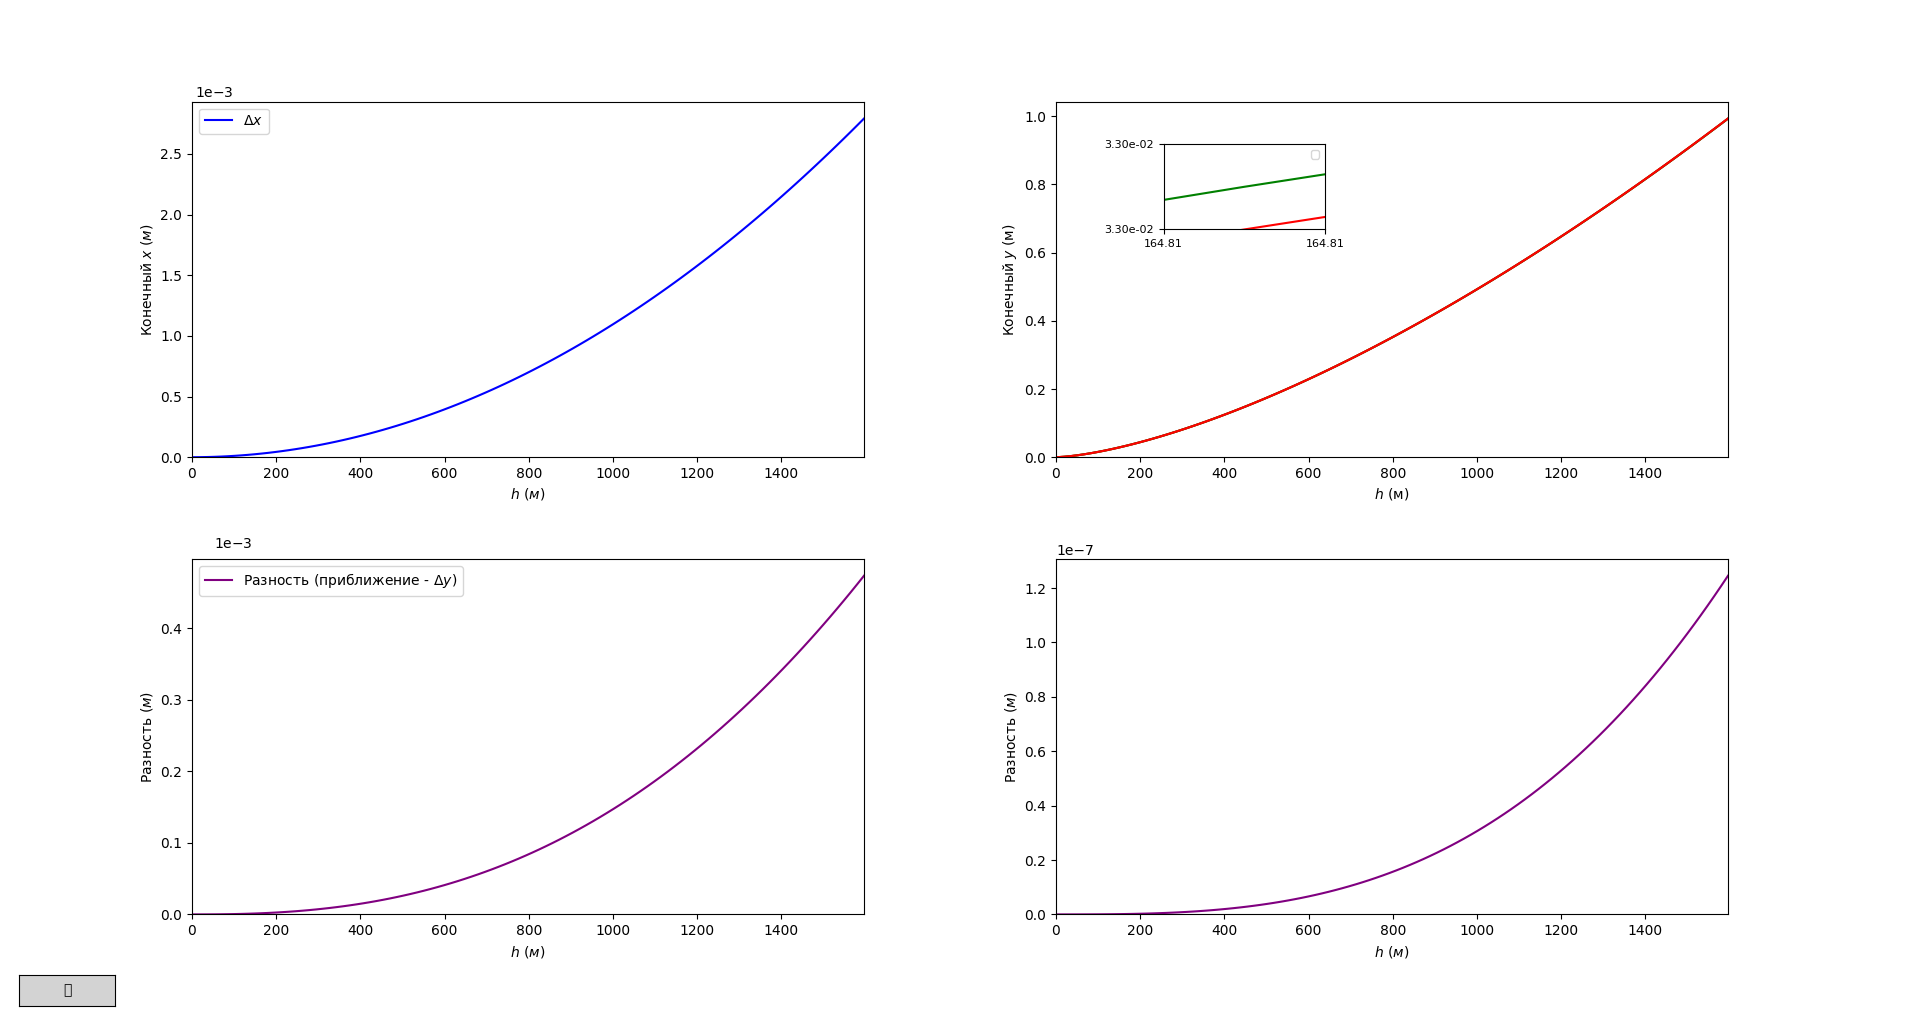
\includegraphics[width=1\textwidth]{fig_1.png}
    \caption{На первом графике показана зависимость смещения по оси $x$. На втором графике зависимость смещения по оси $y$, зеленым цветом показано численное решение дифференциального уравнения, а красным аналитическое. На третьем графике показана разность аналитического решения и численного по оси $y$. На четвертом графике показана разность аналитического решения и численного по оси $x$. С начальными параметрами $v=0$, $\psi=45^{\circ}$, бросок происходил с поверхности земли}
\end{figure}
\begin{figure}[H]
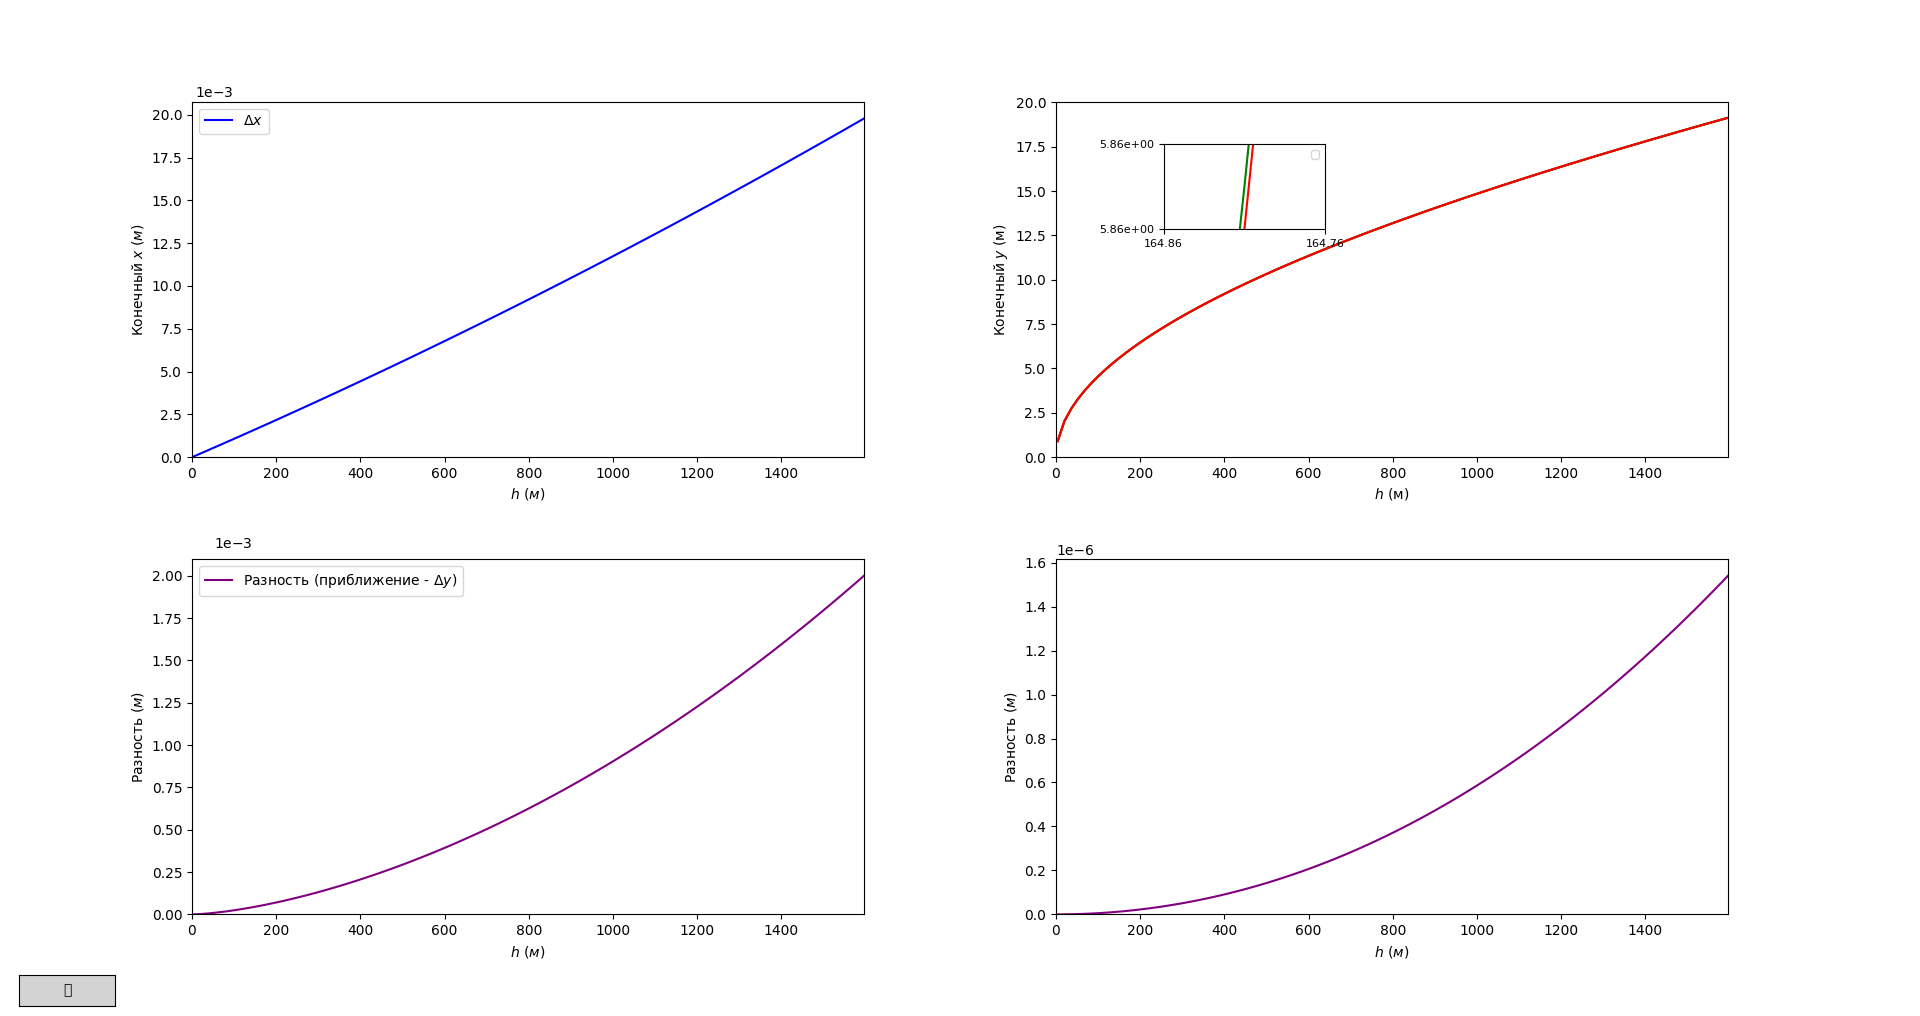
\includegraphics[width=1\textwidth]{fig_2.png}
    \caption{На первом графике показана зависимость смещения по оси $x$. На втором графике зависимость смещения по оси $y$, зеленым цветом показано численное решение дифференциального уравнения, а красным аналитическое. На третьем графике показана разность аналитического решения и численного по оси $y$. На четвертом графике показана разность аналитического решения и численного по оси $x$. С начальными параметрами $v=1$, $\psi=45^{\circ}$, бросок происходил с поверхности земли}
\end{figure}
\begin{figure}[H]
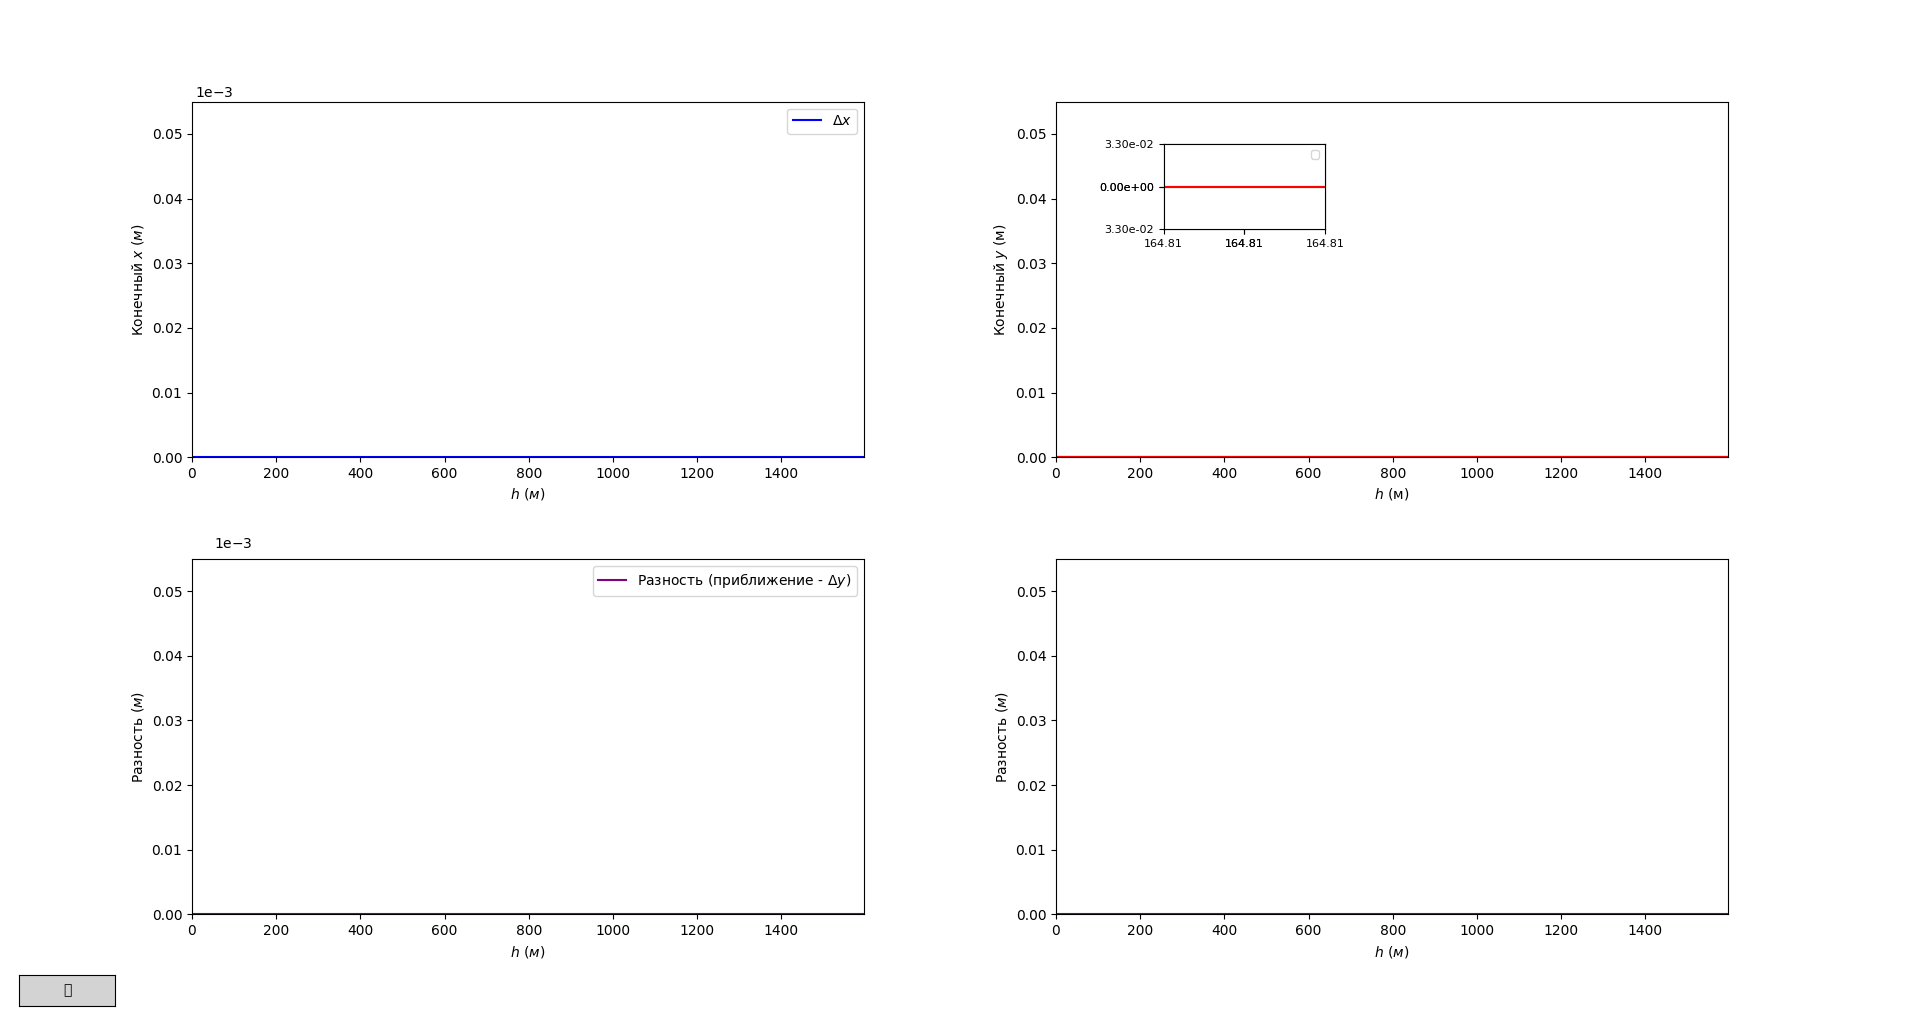
\includegraphics[width=1\textwidth]{fig_3.png}
    \caption{На первом графике показана зависимость смещения по оси $x$. На втором графике зависимость смещения по оси $y$, зеленым цветом показано численное решение дифференциального уравнения, а красным аналитическое. На третьем графике показана разность аналитического решения и численного по оси $y$. На четвертом графике показана разность аналитического решения и численного по оси $x$. С начальными параметрами $v=0$, $\psi=0^{\circ}$, бросок происходил с поверхности земли}
\end{figure}
\begin{figure}[H]
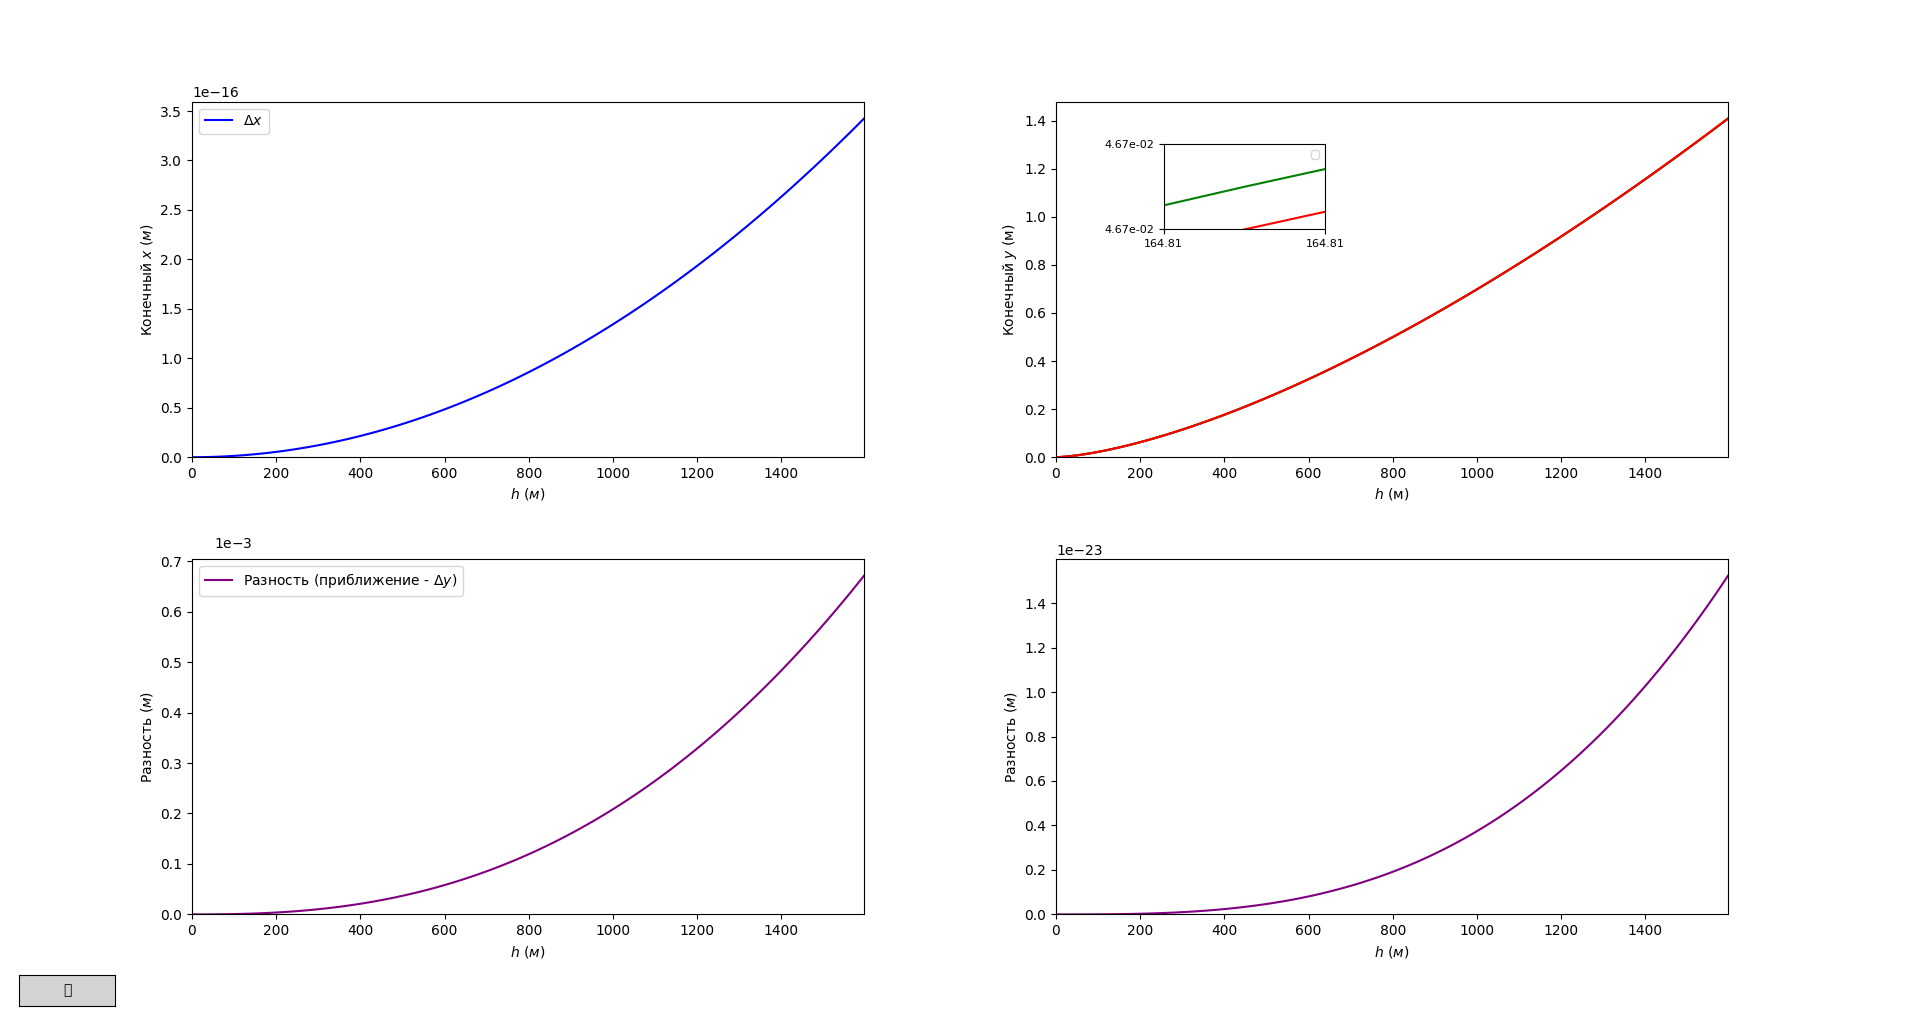
\includegraphics[width=1\textwidth]{fig_4.png}
    \caption{На первом графике показана зависимость смещения по оси $x$. На втором графике зависимость смещения по оси $y$, зеленым цветом показано численное решение дифференциального уравнения, а красным аналитическое. На третьем графике показана разность аналитического решения и численного по оси $y$. На четвертом графике показана разность аналитического решения и численного по оси $x$. С начальными параметрами $v=0$, $\psi=90^{\circ}$, бросок происходил с поверхности земли}
\end{figure}

\twocolumngrid
\section{Заключение}
\bibliography{plus} 
\newpage
\onecolumngrid
\textbf{Приложение А: Вывод дифференциальной системы уравнений.\cite{4}-?}\\
В неинерциаольной системе отсчета связанной с Землей второй закон Ньютона принимает следующий вид:
\begin{equation}
\bm{a}=\dfrac{\bm{F}}{m}-\bm{a}_{EC}-\bm{\omega} \times(\bm{\omega}\times \bm{R}) -2\bm{\omega} \times \bm{v}\text{,}\label{eq:1}
\end{equation}
где $\bm{a}_{EC}$  --- ускорение центра земли, $\bm{\omega}$  --- скорость осевого вращения Земли, считаем что ${\dot\omega}=0$, $\boldsymbol{F}/m$ --- суммарная внешняя сила на массу тела.\\
Перепишем в виде:
\begin{equation}
\bm{a}=\dfrac{\bm{F_{ng}}}{m}+\bm{g}+\bm{a_{cor}},\label{eq:2}
\end{equation}
где $\bm{F_{ng}}$ --- внешняя не гравитационная сила;
\begin{equation*}
    \bm g=\bm{g_E}+\bm{g_{\omega}}+\bm{g_T},
\end{equation*}
 где $\bm{g_E}$ --- ускорение от гравитационного поля земли, $\bm{g_{\omega}}$ ---  центростремительное ускорение, $\bm{g_T}$
--- эффективное гравитационное поле, то есть разность между внешним полем в точке расположения тела и в центре Земли.\\
Из рис.~\ref{fig:pick-1} понятно, что $\bm{R}=\bm{R_0}+\bm{r}$, из выбранных осей следует, что $\bm{g_{0z}}=-g_0\bm{k}$, $g_{0x}=g_{0y}=0$, где $\bm{k}$ - это единичный вектор, направленный вдоль оси $z$.\\
Разложим вектор $\bm{g}$ на две составляющие $\bm{g_0}$ и $\Delta\bm{g}$, где $\bm{\Delta\bm{g}}$ --- это отклонение $\bm{g}$ от его локального значения в точке отсчета. Кроме того, анализ значительно упрощается и сопровождается пренебрежимо малой погрешностью для достаточно локальных движений, если учитывать только изменение $\bm{g}$ первого порядка относительно $\bm{r}$, то есть заменить $\Delta \bm g=\delta \bm g=\bm r \cdot \nabla_0 \bm g$, где индекс «0» указывает, что градиент рассчитывается в локальной точке отсчета
\begin{align}
&\bm a = \dfrac{\bm{F_{ng}}}{m}+\bm{g_0}+\delta\bm g+\bm{a_{cor}}\text{,} \label{eq:3}\\
&\bm{g_0}=-g_0\bm k \text{,} \label{eq:4}\\
&\delta\bm g=\bm r\cdot grad \ \bm g\text{,}\label{eq:5}
\end{align}

\begin{figure}[h]
\centering
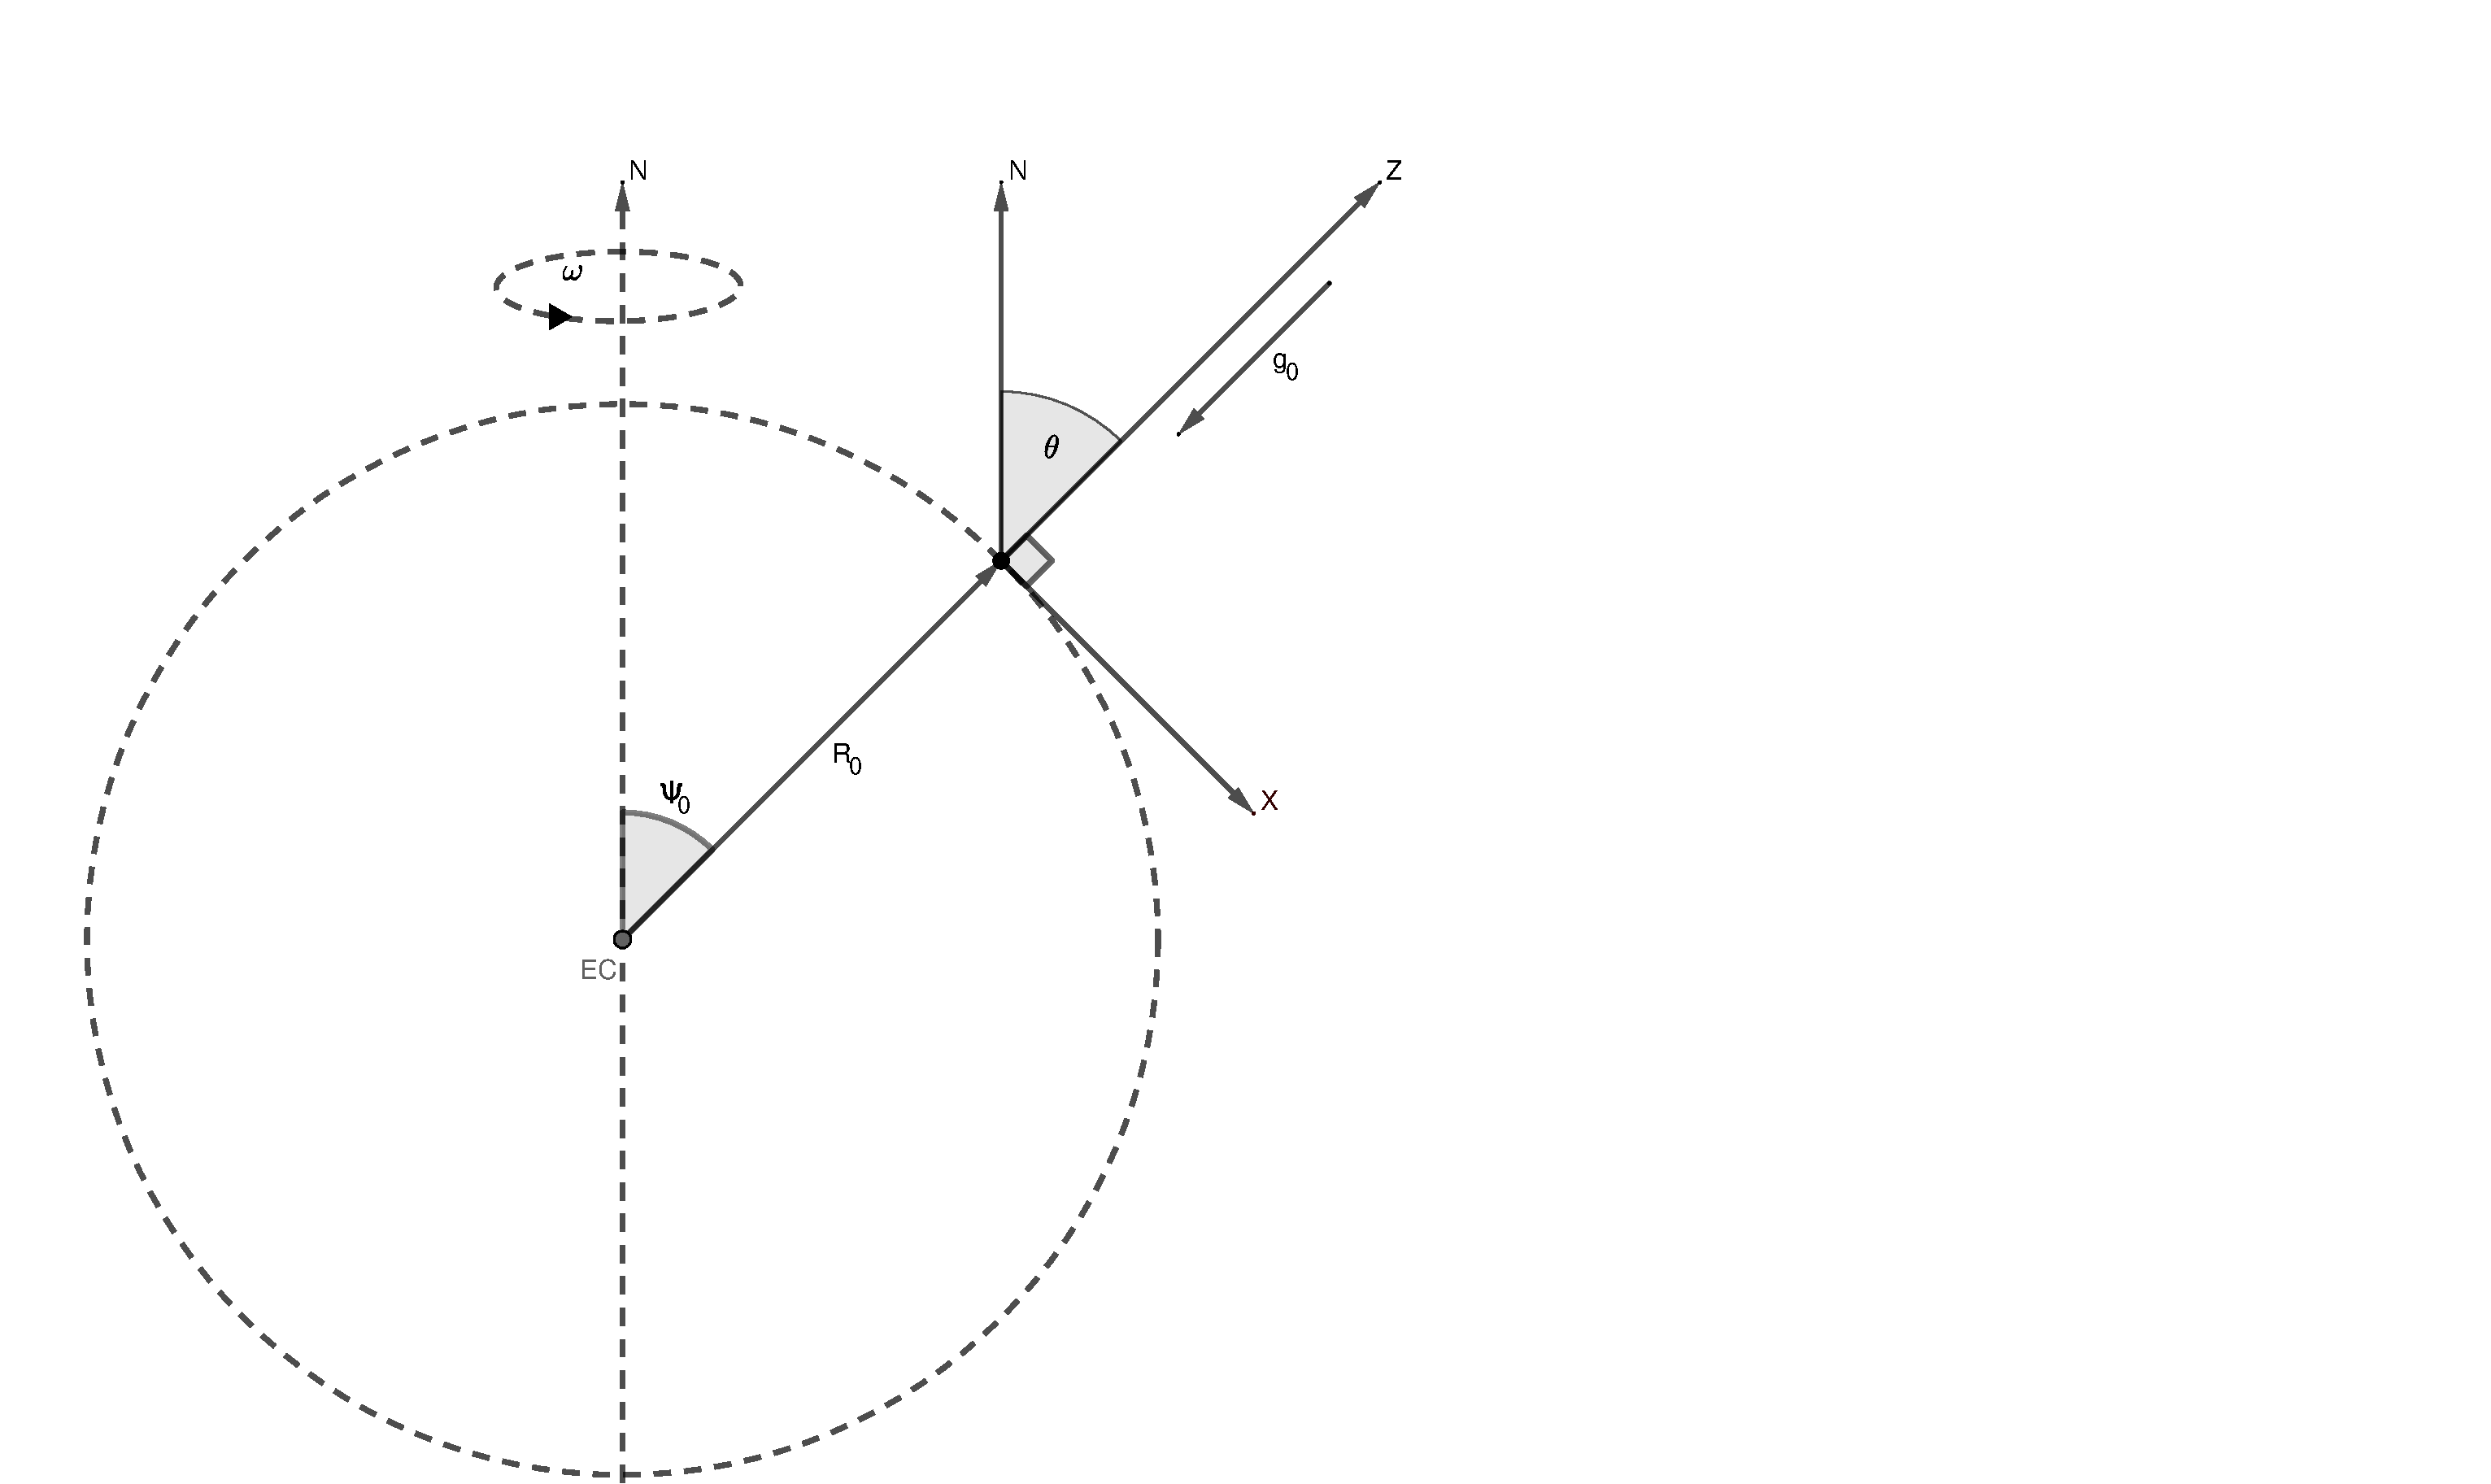
\includegraphics[width=0.4\textwidth]{pick-1.pdf}
\caption{$N$ --- ось вращения планеты, $EC$ --- центр земли, ось $x$ направлена к экватору и  лежит в плоскости, образованной вертикальной осью $z$ и меридианом, который проходит через точку пересечения оси $z$ и поверхностью планеты. Ось $y$ направлена на восток. $\theta$ --- угол между осью вращения $N$ и осью $z$. Местом броска задаются $M$, $R_0$, $\omega$ --- масса, радиус и  угловая скорость вращения планеты соответственно; $\psi_0$ --- угол между северным полюсом и местом броска. $g_0$ --- локальное начальное значение ускорения свободного падения в точке отсчета. $R$ и $r$ --- радиус-векторы брошенного тела относительно центра планеты $EC$ и начала системы координат соответственно.}
\label{fig:pick-1}
\end{figure}

Разложим $\delta\bm g$ и $\bm{a_{cor}}$ на компоненты:

\begin{equation}
    \begin{aligned}
        &\delta g_{\mu} = g_{\mu, x}x + g_{\mu, y}y+g_{\mu,z}z,\\
        &g_{\mu, \nu}=\dfrac{\partial g_{\mu}}{\partial \nu},\\
    & \mu,\nu = x, y, z. \label{eq:6}
    \end{aligned}
\end{equation}
\begin{subequations}
    \begin{align}
        &\boldsymbol{\omega} = \omega_x\hat{\mathbf{i}}  + \omega_z\hat{\mathbf{k}}, \quad \omega_x = -\omega\sin{\theta}, \quad \omega_z = \omega\cos{\theta} \label{eq:7a}\\
        &\boldsymbol{a}_{Cor} = 2\omega_z\dot y\hat{\mathbf{i}} + (2\omega_x\dot z - 2\omega_z\dot x)\hat{\mathbf{j}}-2\omega_x\dot y\hat{\mathbf{k}}.\label{eq:7b}
    \end{align}
\end{subequations}

\begin{equation}
    \boldsymbol{g}_E = -\dfrac{GM_E}{R^2}\hat{\mathbf{R}} = -\dfrac{GM_E}{R^3}{\mathbf{R}},\label{eq:8}
\end{equation}


где частные производные в уравнении (\ref{eq:6}) вычисляются в локальной точке начала отсчёта.  При использовании уравнения (\ref{eq:3}), (\ref{eq:4}), (\ref{eq:5}) значение $g_0$ может быть либо измеренно (гравиметр $g_0$ и отвес для $\theta$), либо вычесленно на основе сферической модели идеально гладкой Земли.

В любой конкретной задаче необходимо определиться с желаемой точностью результата, чем можно, а чем нельзя пренебрегать в конкретном случае. При рассмотрении вертикально падающих объектов с высоты до 100 м, вертикальная состовляющая движения с высокой точностью описывается в предположении однородности гравитационного поля; для восточного отклонения необходимо учитывать ускорение Кориолисса (с точностью до первого порядка $\omega$); для рассчета меридиального движения требует учета уже второго порядка $\omega^2$, а также градиента $g_{x,z}$ первого порядка. Кроме того, значения $g_{x,z}$, рассчитанные для модели идеально сферической Земли также могут отличаться от реального локального значения на порядок \cite{4}.НОРМАЛЬНО ПЛАВНО ПЕРЕЙТИ
ИЗ-ЗА ПОПРАВОК ТЫРЫ ПЫРЫ...

Количественная обоснованность любого приближения должна быть установлена посредством покомпонентного анализа, с обязательной проверкой порядков величин и/или оценкой вклада как сохраненных, так и пренебрегаемых членов в уравнениях, описывающих динамику системы. Далее будет произведена оценка влияния компонент на вертикально падающее тело.


В модели гладкой сферической Земли, величины $\bm{g_0}$ и $\bm{\delta g}$ получаются из $\bm{g} = \bm{g}_E + \bm{g}_{\omega}$; $\bm{\delta g} = \bm{\delta g}_E + \bm{\delta g}_{\omega}$.

Если считать Землю идеальной сферой с симметричным распределением массы, то поле над ее поверхностью равно:

\begin{equation}
    \boldsymbol{g}_E = -\dfrac{GM_E}{R^2}\hat{\mathbf{R}} = -\dfrac{GM_E}{R^3}{\mathbf{R}}.\label{eq:9}
\end{equation}

Оценка $g_0$ и $\alpha$:

В глобальных сферических координатах, $R, \psi$, центростремительное ускорение  $\bm{g_{\omega}}$  принимает вид:
\begin{equation}
    \bm{g_{\omega}}=\omega^2R(\sin^2{\psi} \boldsymbol{\hat{R_0}}  + \sin{\psi}\cos{\psi}\hat{\psi}),
\end{equation}
 где 
\begin{equation*}
    \hat{\psi} = (\hat{\omega}\times\bm{\hat{R}})\times\bm{\hat{R}}.
\end{equation*} Добавляя это к $\bm{g}_E$, получим следующее:

\begin{equation}
      g_0=-\left(\frac{GM_E}{R_0^2}-\omega^2R_0\sin^2{\psi}\right)\boldsymbol{\hat{R_0}}. \label{eq:10}\
\end{equation}


Выражение (\ref{eq:10}) показывает эффективное ускорение свободного падения в локальной точке. 

Вычисление $\delta g$ и элементов тензора $g_{\mu,\nu}$:

Из $\bm{R} = \bm{R_0} + \bm{r}$, $\bm{g_{\omega}} = - \bm{\omega}\times(\bm{\omega}\times\bm{R})$ и (8) получаем следующее:
\begin{equation}
    \delta \mathbf{g}_\omega=\left(\omega_z^2 x-\omega_x \omega_z z\right) \hat{\mathbf{i}}+\omega^2 y \hat{\mathbf{j}}+\left(\omega_x^2 z-\omega_x \omega_z x\right) \hat{\mathbf{k}}, \label{eq:11}
\end{equation}

\begin{equation}
\delta \mathbf{g}_E=3 \frac{G M_E}{R_0^4} \mathbf{R}_0 \delta R -\frac{G M_E}{R_0^3} \delta \mathbf{R},\label{eq:12}
\end{equation}

 где 
\begin{subequations}
\label{eq:13}
    \begin{align}
& \delta R=x \sin \alpha+z \cos \alpha, \label{eq:13a}  \\
& \delta \mathbf{R}=x \hat{\mathbf{i}}+y \hat{\mathbf{j}}+z \hat{\mathbf{k}}, \label{eq:13b} \\
& \hat{\mathbf{R}}_0=\sin \alpha \hat{\mathbf{i}}+\cos \alpha \hat{\mathbf{k}}. \label{eq:13c}
\end{align}
\end{subequations}
В (\ref{eq:12}) и (\ref{eq:13}) заменим $\sin{\alpha} \approx \alpha$, $\cos{\alpha} \approx 1$ и пренебрегая $\alpha^2$ (погрешность $\alpha^2$ порядка $10^{-5}$), получим следующее выражение для $\delta\bm{g_E}$:
\begin{equation}
    \delta g_E=\dfrac{g_{E0}}{R_0}[ (-x+3\alpha z)\hat{\boldsymbol{i}}-y\hat{\boldsymbol{j}}+(3\alpha x+2z)\hat{\boldsymbol{k}}].\label{eq:14}
\end{equation}

Используя (\ref{eq:6}), (\ref{eq:11}) и (\ref{eq:14}), подставляя необходимые компоненты в $g_{\mu , \nu} (\mu, \nu = x, y$ или $z$), получаем компоненты для тензора. Значения следующие:

\begin{subequations}
\label{eq:15}
    \begin{align}
        &g_{x,x}=-\left(\dfrac{g_{E0}}{R_0}-\omega_z^2\right),\label{eq:15a} \\
    &g_{y,y}=-\left(\dfrac{g_{E0}}{R_0}-\omega_y^2\right),\label{eq:15b} \\
    &g_{z,z}=2\dfrac{g_{E0}}{R_0}+\omega_x^2, \label{eq:15c}\\
    &g_{x,z}=g_{z,x}=3\alpha\dfrac{g_{E0}}{R_0} - \omega_x\omega_z,\label{eq:15d}\\
    &g_{x,y}=g_{y,x}=g_{y,z}=g_{z,y}=0.\label{eq:15e}
    \end{align}
\end{subequations}

Выражение (\ref{eq:15e}) справедливо для модели сферичной гладкой Земли. Кроме того, порядки велечин $g_{\mu, \nu}$:

\begin{equation}
     |g_{x,x }|\approx |g_{y,y}| \approx g_{z,z} \approx \dfrac{g_{E0}}{R_0}\approx 10^{-6}s^{-2},\quad
    g_{x,z} = g_{z,x} \approx \omega^2 \approx 10^{-8}s^{-2}.\label{eq:16}
\end{equation}


Падение вертикально падающего тела.

Приняв в (6) $\bm{F_{ng}} = 0$ и использовав (\ref{eq:7b}) и (\ref{eq:15}) получим следующие уравнение движения по $x, y, z$ при использовании сферической модели Земли:

\begin{subequations}
\label{eq:17}
    \begin{align}
       \ddot{x} &= g_{x, x}x +g_{x,z}z+2\omega_{z}\dot{y}, \label{eq:17a}\\
    \ddot{y} &= g_{y, y}y -2\omega_{z}\dot{x} +2\omega_{x}\dot{z},\label{eq:17b} \\
     \ddot{z} &= - g_0+ g_{z, x}x + g_{z, z}z-2\omega_{x}\dot{y}.\label{eq:17c} 
    \end{align}
\end{subequations}
\end{document}
